\chapter{Introduction}
\label{Introduction}

\begin{quote}
\textit{The dissertation is first presented by contextualizing the scientific background of CERN and LIP organizations, as well as their current research projects, which are closely involved in this work. The motivation for the dissertation is presented in section \ref{Motivation}, with the problem contextualized from a physics perspective in subsection \ref{TopQuarkSystem}. The Goals, subsection \ref{Goals}, states the objectives to be achieved by this work, in terms of improving the research and application development quality by implementing a set of solutions for homogeneous and heterogeneous systems, while assessing the efficiency and usability of hardware accelerators in the latter. The scientific contribution of this work is presented in subsection \ref{ScientificContribution}. Subsection \ref{DissertationStructure} overviews the structure of this dissertation.}
\end{quote}

\section{Context}
\label{Context}

Today's computing platforms are becoming increasingly complex with the introduction of multiple multicore CPU chips per system, sometimes coupled with hardware accelerators. While the application performance is an important issue to tackle, the efficient usage of the resources of these systems is a crucial subject that is becoming increasingly popular. Guaranteeing that the available computational resources are being fully used by an application requires extensive knowledge of the underlying architecture details of both CPUs and hardware accelerators. It is important to understand the resources on a CPU, such as computational units organization, benefits and limitations of using multiple cores, and cache memory hierarchy, to avoid underusing the full computational potential of the chip. The architecture design of many-core hardware accelerators have significant differences from chip to chip with no standard yet defined, unlike CPUs. The programmer must know the architectural details of each hardware accelerator for producing efficient code. From the hardware point of view, efficiency may also translate in the ratio between power usage and computational performance.

The memory organization varies between homogeneous and heterogeneous systems, where the first use a shared memory paradigm and the latter a distributed memory paradigm. This means that the data is always available for the CPUs on a system but, when considering hardware accelerators that are coupled by a PCI-Express interface, data must be explicitly passed between CPU and device. The management of the data may affect the performance and efficiency of an application if it causes startvation of the resources. Parallelism is often used to take advantage of the multiple cores in both the CPUs and the hardware accelerators, with the programming paradigm differing from shared to distributed memory environments. Data races, resource contention and, in heterogeneous systems, explicit memory transfers are complex issues that the programmer must tackle. Also, each accelerator manufacturer uses their own frameworks and compilers for programming their devices. With the current computational systems rapidly changing, scientists restrain from investing on academic formation in computer science, opting for self-learning these complex principles. These factors reinforced the collaboration of multidisciplinary teams of scientists from various fields with computer scientists to develop high performing, efficient and robust applications.

The European Organization for Nuclear Research \cite{CERN} (CERN, acronym for \textit{Conseil Européen pour la Recherche Nucléaire}) is a consorcium of 20 european countries, with the purpose of operating the largest particle physics laboratory in the world. Founded in 1954, CERN is located in the border between France and Switzerland, and employs thousands of scientists and engineers representing 608 universities and research groups of 113 different nationalities.

CERN research focus on the basic constituents of matter, which started by studying the atomic nucleus but quickly progressed into high energy physiscs (HEP), namely on the interactions between particles. The instrumentation used in nuclear research is essentially divided into particle accelerators and detectors, alongside with the facilities necessary for delivering the protons to the accelerators. The purpose of the accelerator is to speed up groups of particles close to the speed of light, in opposite directions, resulting in a controlled collision inside the detectors (the collision is called an event). The detectors record various characteristics of the resultant particles, such as energy and momentum, which originate from complex decay processes of the collided protons. The purpose of these experiments is to test and validate specific HEP theories by interpreting the results of the collisions based on the expected theoretical model.

CERN laboratory started with a small low energy particle accelerator, the Proton Synchrotron \cite{CERN:PS} inaugurated in 1959, but soon its equipment was iteratively upgraded and expanded. The current facilities are constituted by the older accelerators (some already decomissioned) and particle detectors, as well as the newer Large Hadron Collider (LHC) \cite{CERN:LHC} high energy particle accelerator, located 100 meter underground and with a 27 km circuference length. There are currently seven experiments running on the LHC: CMS \cite{CERN:CMS}, ATLAS \cite{CERN:ATLAS}, LHCb \cite{CERN:LHCb}, MoEDAL \cite{CERN:MoEDAL}, TOTEM \cite{CERN:TOTEM}, LHC-forward \cite{CERN:LHCf} and ALICE \cite{CERN:ALICE}. Each of these experiments have their own detector on the LHC and conduct HEP experiments, using of distinct technologies and research approaches. One of the most important researches being conducted at CERN is the validation of the Higgs boson theory. The ATLAS experiment, one of the most important projects at CERN, is conducting most of the crucial experiments on both the Top Quark and Higgs Boson theories. During the next year the LHC will be upgraded to increase its luminosity (amount of energy of the accelerated particle beams).

Approximately 600 millions of collisions occur every second at the LHC. Particle detectors react with the particles resultant from the collisions, generating massive amounts of raw data as electric signals. It is estimated that all the detectors combined produce 25 petabytes of data per year \cite{CERN:DATA1,CERN:DATA2}. CERN does not have the financial resources to afford the computational power necessary to process all the data, which motivated the creation of the Worldwide LHC Computing Grid \cite{CERN:WLHCCG}, a distributed computing infrastructure that uses the resources of scientific community for data processing. The grid is organized in a hierarchy divided in 4 tiers. Each tier is made by one or more computing centers and has a set of specific tasks and services to perform, such as store, filter, refine and analyse all the data gathered at the LHC.

The Tier-0 is the data center located at CERN. It provides 20\% of the total grid computing capacity, and its objective is to store and reconstruct the raw data gathered at the detectors in the LHC, converting it into meaningful information, usable by the remaining tiers. The data is received on a format designed for this reconstruction, with information about the event, detector and software diagnostics. The output of the reconstruction has two formats, the Event Summary Data (ESD) and Analysis Object Data (AOD), each with different purposes, containing information of the reconstructed objects and calibration parameters, which can be used for early analysis. This tier distributes the raw data and the reconstructed output by the 11 Tier-1 computational centers, spread among the different countries that are members of CERN.

Tier-1 computational centers are responsible for storing a portion of the raw and reconstructed data and provide support to the grid. In this tier, the reconstructed data suffers more reprocessing, refining and filtering the relevante information and reducing the size of the data, now in Derived Physics Data (DPD) format, then transferred to the Tier-2 computational centers. The size of the data for an event is reduced from 3 MB (raw) to 10 kB (DPD). This tier also stores the output of the simulations performed at Tier-2. The Tier-0 center is connected to the 11 Tier-1 centers by high bandwidth optical fiber links, which form the LHC Optical Private Network.

There are roughly 140 Tier-2 computational centers spread around the world. Their main purpose is to perform both Monte-Carlo simulations and a portion of the events reconstructions, with the data received from the Tier-1 centers. The Tier-3 centers range from university clusters to small personnal computers, and they perform most of the events reconstruction and final data analysis. In the CERN terminology, an analysis is the denomination of an application which is designed to process a given amount of data in order to extract physically relevant information about events that may support a specific HEP theory.

\section{LIP research group}
\label{LIP}

The Laboratório de Instrumentação e Física Experimental de Partículas (LIP) \cite{LIP} is a portuguese scientific and technical association for research on experimental high energy physics and associated instrumentation. LIP has a strong collaboration with CERN as it was the first scientific organization from Portugal that joined, in 1986. It has laboratories in Lisbon, Coimbra and Minho and 170 people employed. LIP researchers have produced several applications for testing various HEP theories of the ATLAS experiment that use Tier-3 computational resources for data analysis. Most of the analysis applications use in-house developed skeleton libraries, such as the LipCbrAnalysis and LipMiniAnalysis.

The motivation for this dissertation, presented in section \ref{Motivation}, results from a close cooperation between the Department of Informatics of the University of Minho and the LIP laboratory in Minho, which began in 2011.

\section{Motivation, goals \& scientific contribution}
\label{Motivation}

With an increase in particle collisions and data being produced by the detectors at the LHC, research groups will need a bigger budget for aquiring and maintaining the required computational resources to keep up with the analysis. Adding to this increase in data, research groups working on the same experiment enforce positive competition to be the first to find and publish relevant results. The amount and quality of event processing as a direct impact on the research, meaning that groups with more computational resources become ahead of the competition.

Better results are not only obtained by increasing the amount of events analyzed; it is important to take into account the quality of each event analysis. The ATLAS detector has an experimental resolution of 2\%, meaning that each measured value for a characteristic of a particle resultant from a collision might not be exact and, therefore, the analysis will have an error associated. It is possible to improve the analysis quality but it will increase its execution time, creating a trade-off between events to analyze and their quality. This issue will be presented in the context of this dissertation in more detail on subsection \ref{TopQuarkSystem}.

One of the most important researches conducted by LIP are related to the discovery of new physics in the Top Quarks and Higgs Boson. An application was devised to reconstruct an event obeying the theoretical model of Top Quark decay. It also attempts to reconstruct the Higgs Boson associated with the event. Each event can be reconstructed several times, with some of its parameters varied by a random offset (with a maximum magnitude of 2\% of the original value), so that a accurate final reconstruction is obtained by chosing the partial reconstruction that better satisfies the theoretical model. The purpose of this mechanism is to overcome the experimental resolution of the ATLAS detector. The number of reconstructions performed per event directly relates to the application execution time. The theoretical model for this system is presented in subsection \ref{TopQuarkSystem} and the analysis application in chapter \ref{Application}.

While investing in the upgrade of the computational resources of the research group is a valid option to deal with the increase of events to analyze, it is also necessary to take into account if the current resources are being efficiently used by the current applications. Also, hardware is not necessarily getting faster, but wider as the number of cores per chip is increasing rather that its speed (see chapter \ref{TechnologicalBackground}), which can cause big investments to result in small improvements. Current computing clusters are constituted of systems with one or more multicore CPUs (homogeneous systems) and some coupled with hardware accelerators, which are very fast and efficient for specific problem domains (heterogeneous systems). It is important to have a knowledge of the newer architectures in order to develop efficient applications that resort to parallelism to efficiently use the system resources. Programming for such architectures (both multicore CPUs and hardware accelerators) requires a set of skills and experience that most physicists (usually self-taught programmers) lack, which causes developed applications to not use the full potential of these systems.

Increasing the efficiency of an application by resorting to parallelism enables the possibility of performing more reconstructions per event and more events to be processed, while using all the potential of the available computational resources and avoiding needless investments in hardware upgrades.

\subsection{The top quark system and Higgs boson decay}
\label{TopQuarkSystem}

In the LHC, two proton beams are accelerated close to the speed of light in opposite directions, set to collide inside a specific particle detector. From this head-on collision results a chain reaction of decaying particles, and most of the final particles react with the detector allowing their characteristics to be recorded. One of the experiments being conducted at the ATLAS detector is related to the discovery of new Top Quark physics. The schematic representation of the Top Quark decay (usually addressed as the \ttbar system), resultant from a head-on collision of two protons, is presented in figure \ref{fig:TopQuarkDecay}.

\begin{figure}[!htp]
	\begin{center}
		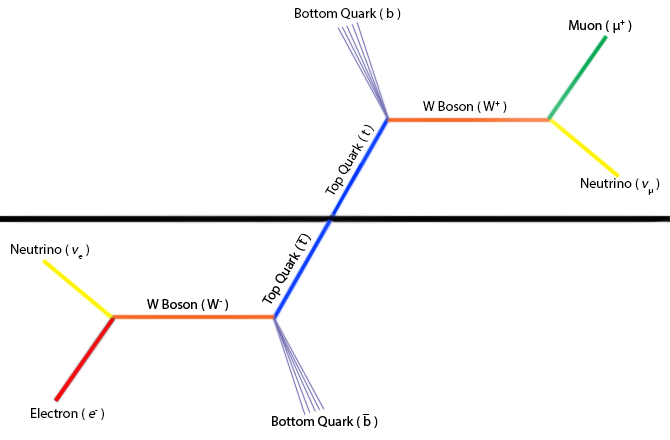
\includegraphics[scale=0.5]{../../common/img/ttbar.png}
		\caption{Schematic representation of the \ttbar system.}
		\label{fig:TopQuarkDecay}
	\end{center}
\end{figure}

The ATLAS detector is able to record the characteristics of Bottom Quarks, detected as a jet of particles, and leptons, the muon (with a positive charge) and electron (with a negative charge). However, the neutrinos do not react with the detector and, therefore, their characteristics are not recorded. To reconstruct the Top Quarks it is necessary to have the information of all the final particles, so the neutrino characteristics need to be determined. The neutrinos characteristics can be analitically calculated with the information of the quarks and leptons, using a set of properties that determine the behavior of the \ttbar system. The process of reconstructing the neutrinos is referred as kinematical reconstruction. The reconstruction of the whole \ttbar system has a degree of certainty associated, which determines its quality. The quality of these reconstructions directly impact the research outcome.

The amount of Bottom Quark jets and leptons detected may vary between events, due to other reactions occurring simultaneously to the Top Quark decay. As represented in figure \ref{fig:TopQuarkDecay}, 2 jets and 2 leptons are needed to reconstruct the \ttbar system, but the input data for an event may have many more of these particles associated. It is necessary to reconstruct the neutrinos, and then the whole system, for every combination of 2 jets and 2 leptons (often referred only as \textit{combination}) available in the input data and only chose the most accurate reconstruction, for each given event.

Another factor affecting the quality of the reconstruction is the experimental resolution of the ATLAS particle detector, which associates an error up to 2\% with every measurement made. If the measurements of the jets and leptons are not precise enough the kinematical reconstruction will produce inaccurate neutrinos and affect the overall reconstruction of an event. This might render an event useless that otherwise would provide relevant physics information. It is possible to overcome this problem by performing the whole \ttbar system reconstruction a given amount of times for each combination of 2 Bottom Quark jets with 2 leptons, randomly varying the particle characteristics (momentum, energy and mass), with a maximum magnitude of 2\% of the original value. The amount of variations performed per combination will directly proportional the final quality of the event reconstruction, as more of the search scope (defined by the experimental resolution error) is covered, compared to performing a single \ttbar system reconstruction.

The search for the Higgs Boson is also part of the research being conducted at LIP. Figure \ref{fig:HiggsBosonDecay} schematizes the Higgs Boson and Top Quark decay. It is possible to reconstruct the Higgs Boson from the two Bottom Quark jets that it decays to, and it can be performed alongside the \ttbar system reconstruction. This adds at least two more jets to the event information, and it is not possible to know before the reconstruction which jets belong to the Higgs decay or the Top Quark decay. The Higgs reconstruction must be performed after the \ttbar system reconstruction, in such a way that the jets chosen to reconstruct it must not be the ones used in the \ttbar system reconstruction. Adding this new jets increases the number of jets/leptons combinations to test in the kinematical reconstruction, and the Higgs Boson must be always reconstructed for each \ttbar system. The overall quality of the event reconstruction depends on the quality of both \ttbar system and Higgs Boson reconstructions.

\begin{figure}[!htp]
	\begin{center}
		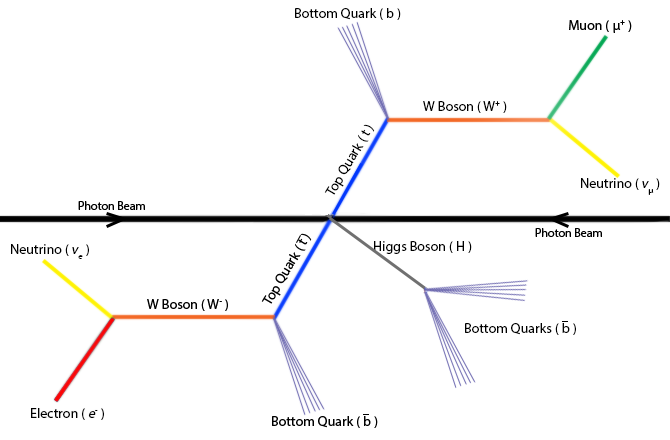
\includegraphics[scale=0.5]{../../common/img/ttbar_higgs.png}
		\caption{Schematic representation of the \ttbar system with the Higgs Boson decay.}
		\label{fig:HiggsBosonDecay}
	\end{center}
\end{figure}

The analysis presented in this section is performed by the \tth application developed by LIP researchers. The application receives input data file with a set of event data and attempts to reconstructs both the \ttbar system and the Higgs Boson of each event, using the processes described. These files are usually 1 GB long and the LIP process huge quantities using this application for the research on Top Quark and Higgs Boson physics. A in-depth computational analysis of \tth is presented in chapter \ref{Application}, where its flow is presented, computationally characterized and the critical region affecting the performance is identified.

\subsection{Goals}
\label{Goals}

\tth is expected to perform more variations per event by improving the performance of the Top Quark and Higgs Boson reconstructions, boosting the quality of the results, within the same, or less, time that the current non-varied event processing occurs. The objective of this dissertation is to take the \tth scientific application coded by physicists, which the main concern during its development was the correcteness of the code rather than its performance, and improve its efficiency by (i) identifying the bottlenecks and optimizing the code, (ii) increasing the performance by resorting to parallelism for homogeneous and heterogeneous systems, assessing the performance and usability of hardware accelerators for this type of problem, and (iii) the development of a simple scheduler for managing the workload distribution among various instances of the same sequential or parallel application (i.e., an application which needs to process a large set of separate input files) on homogeneous systems, without changes to the application.

This work will give a inside perspective of how scientific applications are being developed by self taught programmers with no background in computer science, and help define a set guidelines for coding efficient applications for complex parallel systems. All the changes that will be made to the \tth application, including the introduction of parallelism, are as modular as possible from the context of this specific application, in such a way that they are portable to other applications, requiring small changes to the code. The scheduler will offer parallelization of the data to process at the application level, requiring no changes to the application source code. The implementations will be structured so that the parallelization mechanisms and the scheduler can be improved to be later improved into the LIP libraries to produce a tool that automatically extracts parallelism from these applications, without LIP researchers needing to deal with the complexities of efficient programming for these systems.

\subsection{Scientific contribution}
\label{ScientificContribution}

This dissertation work aimed to improve the performance, efficiency and quality of an analysis application. The application is now able to process more variations and events by efficiently using the computational resources on a system. This improves the quality of the research conducted by LIP on the Top Quarks and Higgs Boson, without requiring any investments in hardware. The application scheduler is designed to work with any kind of application, extracting parallelism from simultaneous executions of applications, leading to a more efficient resource usage, which can improve the performance of all LIP applications.

The expertise gained from parallelizing this kind of complex applications on both homogeneous and heterogeneous systems allowed to provide a set of guidelines for restructuring the LipMiniAnalysis library that, allied to the application scheduler, can be transformed into a tool that automatically extracts parallelism from LIP applications.

\section{Dissertation structure}
\label{DissertationStructure}

This dissertation has 5 chapters with their summary presented below:

\begin{description}
	\item[Introduction] \hfill \\
	The dissertation is first presented by contextualizing the scientific background of CERN and LIP organizations, as well as their current research projects, which are closely involved in this work. The motivation for the dissertation is presented in section \ref{Motivation}, with the problem contextualized from a physics perspective in subsection \ref{TopQuarkSystem}. The Goals, subsection \ref{Goals}, states the objectives to be achieved by this work, in terms of improving the research and application development quality by implementing a set of solutions for homogeneous and heterogeneous systems, while assessing the efficiency and usability of hardware accelerators in the latter. The scientific contribution of this work is presented in subsection \ref{ScientificContribution}. Subsection \ref{DissertationStructure} overviews the structure of this dissertation.
	\item[Computing Background] \hfill \\
	This chapter presents the current technological state of the art in terms hardware and software. Hardware-wise, both homogeneous and heterogeneous system architectures and details are presented in sections \ref{HomogeneousSystems} and \ref{HeterogeneousSystems}, respectively. A contextualization of current hardware accelerators is also made in the latter. Software-wise background is presented in section \ref{Software}. Various frameworks and libraries are presented for homogeneous systems and accelerators in sections \ref{pThreads}, \ref{OpenMP}, \ref{MPI} and \ref{CUDA}. Section \ref{HeterogeneousFrameworks} presents the available frameworks for parallelization in heterogeneous systems. Finally, current solutions for profiling and debugging parallel applications is presented in section \ref{ProfilingDebugging}.
	\item[Top Quark and Higgs Boson reconstructions] \hfill \\
	The \tth application for event reconstruction is presented in this chapter. Its dependencies are presented. The flow of the application is presented in section \ref{Application:Flow}, accompanied by a schematic representation. Its main functions are presented and the schematic flow is compared against a callgraph of the application to help understanding what happens in each of the most important functions. The critical region is identified in section \ref{CriticalRegion} and characterized in subsection \ref{ComputationalCharactrization}. Some initial optimizations to the code are presented in subsection \ref{InitialOptimizations}.
	\item[Parallelization Approaches] \hfill \\
	For different parallelization alternatives are presented in this chapter. For homogeneous systems, a shared memory parallelization is discussed in section \ref{Parallelization:SharedMem}, where the abstract heuristic used is shown, and the implementation and a performance analysis are presented in subsections \ref{SharedMemImplementation} and \ref{SharedMemPerformance}, respectively. For heterogeneous systems using hardware accelerators, two alternatives are presented: using GPU as an accelerator, in section \ref{Parallelization:GPU}, with its implementation and performance discussed and analyzed in subsections \ref{GPUImplementation} and \ref{GPUPerformance}; using the \intel Xeon Phi as an accelerator in section \ref{Parallelization:MIC} and its implementation discussed in subsection \ref{MICImplementation}. A software scheduler for managing workload distribution among applications for homogeneous shared memory systems is presented in section \ref{Parallelization:Scheduler}. Its implementation details and performance analysis are shown in subsections \ref{SchedulerImplementation} and \ref{SchedulerPerformance}.
	\item[Conclusions \& Future Work] \hfill \\
	This chapter concludes the dissertation, presenting an overview of the results obtained by the work developed, on both homogeneous and heterogeneous systems. Guidelines for future work, on improving the test case application and providing parallel solutions abstracted from the programmer for future application development, are presented.
\end{description}
